%%This is a very basic article template.
%%There is just one section and two subsections.
\documentclass{article}
\usepackage{a4wide}
\usepackage{amsmath}
\usepackage{float}
\usepackage{graphicx}
\usepackage{listings}
\usepackage{tikz}
\usetikzlibrary{shapes,snakes}

\begin{document}

\title{Data Mining\\ Exercise 2}
\author{Charalampos Kaidos}

\maketitle

\section*{Data model}

The data model in the graph database consists of 3 nodes. A node describing the
player of the game, a node describing the game and a node describing each
position of the chess board during the game.

The player node has one attribure, the name of the player. The game has several
attributes: the date of the game, the number of halfmoves, the number of moves,
the result (winner) of the game, the number of the game in the data set, the
event that the game was part of, the place where the game took place, the date
the event started, the round of the event that this game was played for, the ECO
code of the opening and the description of the opening. Finally, the position
node has 2 attributes, the position number within the game and the FEN, which is
an ASCII description of the state of the board.

The nodes are interconnected with relationships. A relationship called either
plays, with 2 attributes; color and elo discribes how a player takes part in a
game. A relationship called contains expresses the containement of a position in
a game. Finally a relationship called move expresses the piece movement that
transitioned the game from one board position to another. The move relationship
has 2 attributes: the move and the side that performed the move.

\begin{figure}[H]
\centering
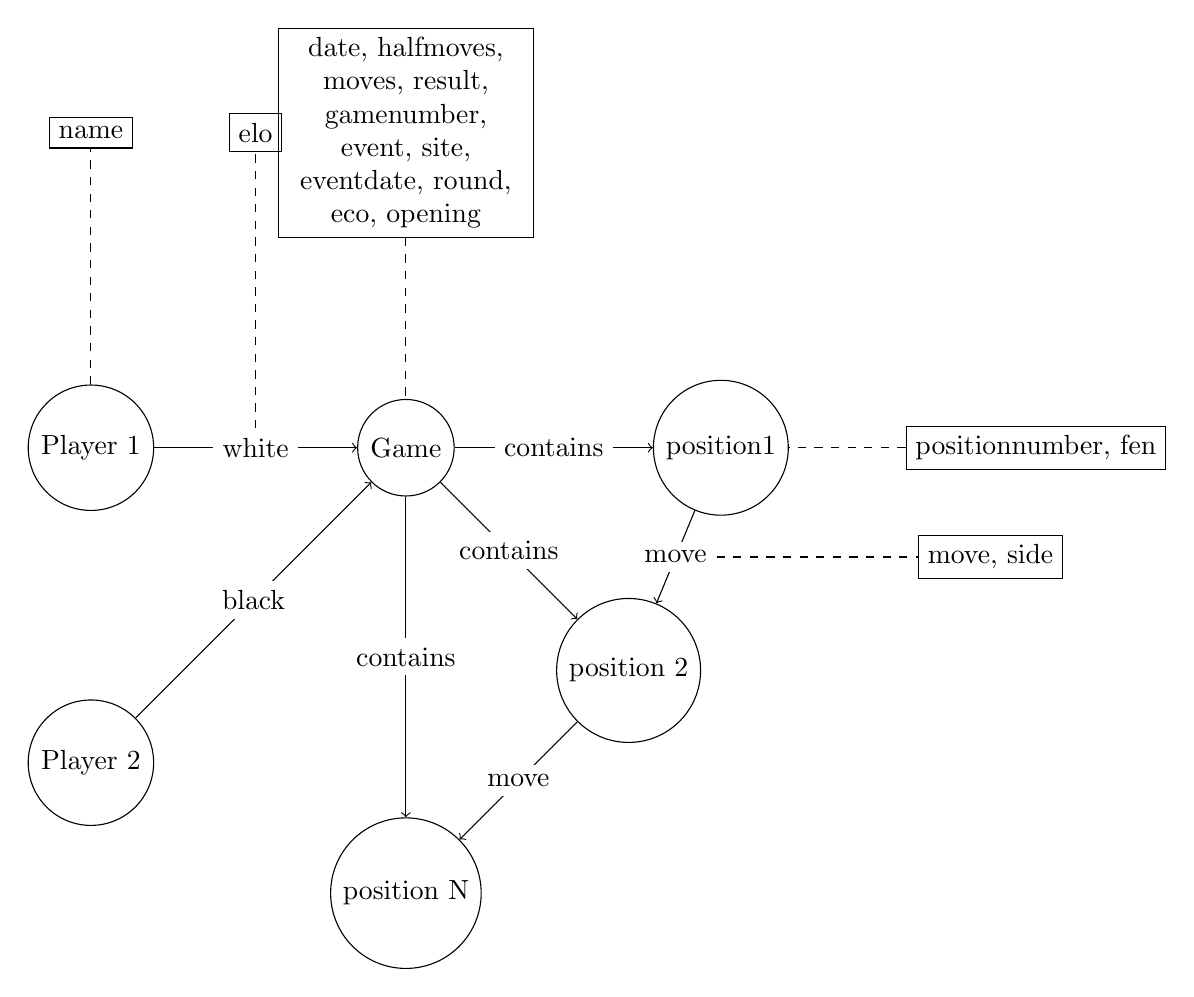
\begin{tikzpicture}[node distance=4cm]
\tikzstyle{cir} = [circle,draw=black,fill=none]
\tikzstyle{rec} = [rectangle,draw=black,fill=none]

\node[cir](game)			{Game};
\node[rec](gamedata)[above of=game][text width=3cm,align=center]		{date,
halfmoves, moves, result, gamenumber, event, site, eventdate, round, eco, opening};
\node[cir](position1)[right of=game]			{position1};
\node[rec](posdata)[right of=position1]		{positionnumber, fen};
\node[cir](position2)[below right of=game]			{position 2};
\node[cir](positionn)[below left of=position2]			{position N};
\node[cir](player1)[left of=game]			{Player 1};
\node[cir](player2)[below of=player1]			{Player 2};
\node[rec](playerdata)[above of=player1]			{name};

\draw [->] (game) -- (position1) node [midway, fill=white] {contains};
\draw [->] (game) -- (position2) node [midway, fill=white] {contains};
\draw [->] (game) -- (positionn) node [midway, fill=white] {contains};
\draw [->] (position1) -- (position2) node(m1) [midway, fill=white] {move};
\draw [->] (position2) -- (positionn) node [midway, fill=white] {move};

\draw [->] (player1) -- (game) node(w1) [midway, fill=white] {white};
\draw [->] (player2) -- (game) node [midway, fill=white] {black};

\node[rec](movedata)[right of=m1] {move, side};
\node[rec](whitedata)[above of=w1] {elo};

\draw [dashed,-] (gamedata) -- (game);
\draw [dashed,-] (posdata) -- (position1);
\draw [dashed,-] (m1) -- (movedata);
\draw [dashed,-] (w1) -- (whitedata);
\draw [dashed,-] (player1) -- (playerdata);

\end{tikzpicture}
\end{figure}

In order to insert the chess games data in Neo4j we had to tranform them to CSV
format. We wrote a small python script for that, which you can find in
chess\_to\_csv.py. The script produces 2 csv files, one containing
information about the games and pleyers and another one containing data abour the moves that
took place in each game.

The games data (chessData\_games.csv) contains 15 columns: white, black,
date, halfmoves, moves, result, whiteelo, blackelo, gamenumber, event, site,
eventdate, round, eco, opening. The moves data (chessData\_moves.csv) contains 5
columns: movenumber, side, move, fen, gamenumber.

To load the games and players we issue the following script in Cypher:
\begin{lstlisting}
LOAD CSV WITH HEADERS FROM "file:/chessData_games.csv" AS line_game
CREATE (n:Game {date: line_game.date, halfmoves: toInt(line_game.halfmoves), 
	moves: toInt(line_game.moves), result: line_game.result, gamenumber:
	toInt(line_game.gamenumber) , event: line_game.event, site: line_game.site,
	eventdate: line_game.eventdate, round: line_game.round, eco: line_game.eco,
	opening: line_game.opening})
MERGE (p1:Player {name: line_game.white})
MERGE (p2:Player {name: line_game.black})
CREATE (p1)-[w:Plays {side: 'white', elo: line_game.whiteelo}]->(n)
CREATE (p2)-[b:Plays {side: 'black', elo: line_game.blackelo}]->(n)
\end{lstlisting}
This script will create 2 types of nodes, position and player and will connect
them with a relationship with label ``Plays''.

To load the positions we issue the following script:
\begin{lstlisting}
USING PERIODIC COMMIT
LOAD CSV WITH HEADERS FROM "file:/chessData_moves.csv" as line_moves
CREATE (p:Position {positionnumber: toInt(line_moves.movenumber), fen: line_moves.fen,
	gamenumber: toInt(line_moves.gamenumber)})
WITH COLLECT(DISTINCT p.gamenumber) AS pp
FOREACH (gamenu in pp |
	CREATE (p:Position {positionnumber: 0, fen: 
		'rnbqkbnr/pppppppp/8/8/8/8/PPPPPPPP/RNBQKBNR', gamenumber: gamenu}))
\end{lstlisting}
This script will add all positions in the database and also create an initial
position with number 0 for each game.

Next we create indices to speed up the operations that will add relationships to
positions:
\begin{lstlisting}
CREATE INDEX ON :Game(gamenumber);
CREATE INDEX ON :Position(gamenumber);
CREATE INDEX ON :Position(positionnumber);
\end{lstlisting}

Next step is to add the contains relationship between each game and the
positions it contains:
\begin{lstlisting}
USING PERIODIC COMMIT
LOAD CSV WITH HEADERS FROM "file:/chessData_moves.csv" AS line_moves
MATCH (pos:Position {gamenumber: toInt(line_moves.gamenumber)})
MATCH (g:Game {gamenumber: toInt(line_moves.gamenumber)})
MERGE (g)-[:CONTAINS]->(pos);
\end{lstlisting}

Finally we add a move relationship between subsequent positions wihtin a game.
The initial position with number 0 will point to the first position from the
data with the move relationship containing the move that enabled this
transitions. Same for the next positions:
\begin{lstlisting}
LOAD CSV WITH HEADERS FROM "file:/chessData_moves.csv" AS line_move
MATCH (pos1:Position {gamenumber: toInt(line_move.gamenumber), 
	positionnumber: toInt(line_move.movenumber)-1})
MATCH (pos2:Position {gamenumber: toInt(line_move.gamenumber), 
	positionnumber: toInt(line_move.movenumber)})
MERGE (pos1)-[:Move {side: line_move.side, move: line_move.move}]->(pos2)
\end{lstlisting}

\subsection{}
To calculate the number of games where the given position has beed realized and
the ratio of white wins in these games:
\begin{lstlisting}
MATCH (g1:Game)-[:CONTAINS]->(pos:Position {fen: 'r1bqkbnrpppp1ppp2n51B2p34P35N2PPPP1PPPRNBQK2R'})
WITH COUNT(g1) AS c
MATCH (g2:Game {result: 'White'})-[:CONTAINS]->(pos:Position {fen: 
	'r1bqkbnrpppp1ppp2n51B2p34P35N2PPPP1PPPRNBQK2R'})
RETURN c, (count(g2)/1.0)/(c/1.0)
\end{lstlisting}
87 games contain this position and white has won 41\% of them.

\subsection{}
Similar to above, to calculate the ration of draws, black and white wins:
\begin{lstlisting}
MATCH (g1:Game)-[:CONTAINS]->(pos:Position {fen: 'r1bqkbnrpppp1ppp2n51B2p34P35N2PPPP1PPPRNBQK2R'})
WITH COUNT(g1) AS c
MATCH (g2:Game {result: 'White'})-[:CONTAINS]->(pos:Position {fen: 
	'r1bqkbnrpppp1ppp2n51B2p34P35N2PPPP1PPPRNBQK2R'})
WITH COUNT(g2) AS ww, c
MATCH (g3:Game {result: 'Black'})-[:CONTAINS]->(pos:Position {fen: 
	'r1bqkbnrpppp1ppp2n51B2p34P35N2PPPP1PPPRNBQK2R'})
WITH COUNT(g3) AS bw, ww, c
MATCH (g4:Game {result: 'Draw'})-[:CONTAINS]->(pos:Position {fen: 
	'r1bqkbnrpppp1ppp2n51B2p34P35N2PPPP1PPPRNBQK2R'})
WITH COUNT(g4) AS dr, bw, ww, c
RETURN ww*1.0/c AS White_Wins, bw*1.0/c AS Black_Wins, dr*1.0/c AS Draw
\end{lstlisting}
Thus 41\% of wins were for white player, 19\% of wins were for black and 39\%
were draws

\subsection{}
According to the data, the World Championship 31th is the event with most games
and Karpov played in all of them (48)
\begin{lstlisting}
MATCH (g:Game)
WITH DISTINCT g.event AS events, COUNT(g) as game_no
ORDER BY game_no DESC
WITH MAX(game_no) as max_game_no
MATCH (g:Game)
WITH DISTINCT g.event AS events, COUNT(g) as game_no, max_game_no
WITH FILTER (event in events WHERE game_no=max_game_no) as events
MATCH (pl:Player {name: 'Karpov  Anatoly'})-->(g:Game)
WHERE g.event in events
RETURN COUNT(pl), g.event
\end{lstlisting}

\subsection{}
To find the player that has played most games which opened with Ruy Lopez move:
\begin{lstlisting}
MATCH (pl:Player)-[:Plays]->(g:Game {opening: 'Ruy Lopez'})
RETURN DISTINCT pl as pl_name, COUNT(g) as games
ORDER BY games DESC
LIMIT 1
\end{lstlisting}
Lasker Emanuel has played 17 games opening with that move

\subsection{}
The chain of moves Nc6->Bb5->a6 has been played in 104 games by Steinitz 
Wilhelm, Chigorin  Mikhail I, Lasker  Emanuel, Tarrasch  Siegbert, Janowski 
Dawid M, Schlechter  Carl, Alekhine  Alexander A, Bogoljubow  Efim D, Euwe  Max,
Keres  Paul, Reshevsky  Samuel H, Smyslov  Vassily V, Botvinnik  Mikhail M,
Spassky  Boris V, Petrosian  Tigran V, Fischer  Robert J, Korchnoi  Viktor L,
Karpov  Anatoly, Kasparov  Gary:
\begin{lstlisting}
MATCH (pl:Player)-->(g:Game)-->(:Position)-[:Move {move: 'Nc6'}]->(:Position)
	-[:Move {move: 'Bb5'}]->(:Position)-[:Move {move: 'a6'}]->(:Position)
WITH COUNT(g) AS games_no
MATCH (pl:Player)-->(g:Game)-->(:Position)-[:Move {move: 'Nc6'}]->(:Position)
	-[:Move {move: 'Bb5'}]->(:Position)-[:Move {move: 'a6'}]->(:Position)
RETURN DISTINCT pl.name, games_no
\end{lstlisting}

\subsection{}
To view the players that competed in this game:
\begin{lstlisting}
MATCH (pl:Player)-->(:Game {gamenumber: 636})
RETURN pl.name
\end{lstlisting}

To view the data of the game:
\begin{lstlisting}
MATCH (g:Game {gamenumber: 636})
RETURN g
\end{lstlisting}

Finally to view all the moves in order they happened:
\begin{lstlisting}
MATCH p = (g:Game {gamenumber: 636})-->(pos:Position {positionnumber: 0})-[m:Move*]->(pos2:Position)
WITH COLLECT(p) as p, MAX(length(p)) AS maxLength
WITH FILTER(path IN p
	WHERE length(path)= maxLength) AS longestPath, p
Return extract(x IN relationships(longestPath[0]) | x.move)
\end{lstlisting}

\subsection{}


\end{document}
